\subsection{Schnelle Integration in Ruhmannsfelden}

August Högn wurde zum 1.1.1910 an
die Volksschule in Ruhmannsfelden versetzt. \footnote{Dokument Nr. 48,
Zeitungsartikel aus Viechtacher Bayerwald-Bote, 2.8.1958} Der Markt
Ruhmannsfelden, in dem damals ungefähr 1500 Einwohner lebten, liegt im
bayerischen Wald und ist etwa in der Mitte des Dreiecks zu finden, das
die nächst gelegenen drei Städte Viechtach, Regen und Deggendorf
bilden. \footnote{Högn, Ruhmannsfelden, S. 50} Das Einzugsgebiet der
Volksschule umfasste auch vor dem 1. Weltkrieg nicht nur die Gemeinde
Ruhmannsfelden, sondern zusätzlich weite Teile der benachbarten
Gemeinde Zachenberg und Randgebiete der angrenzenden Gemeinde
Patersdorf, also in etwa das Gebiet der Pfarrei St. Laurentius. Die
Gemeinde Zachenberg, die geringfügig mehr Einwohner als Ruhmannsfelden
zählte, bestand aus 38 überwiegend landwirtschaftlich geprägten
Kleinstortschaften und hatte mit dem Dorf Zachenberg kein wirkliches
Zentrum, denn dort bestand weder ein Rathaus noch ein Schulhaus. Nicht
nur in Schulangelegenheiten war Ruhmannsfelden damals wie auch heute
ein Zentrum. Ansässige Ärzte und eine seit 1910 bestehende
Apotheke \footnote{Högn, Ruhmannsfelden, S. 28 – 29} lieferten auch für
die Bewohner der Nachbargemeinden Achslach und Gotteszell einen Grund,
Ruhmannsfelden zu besuchen.


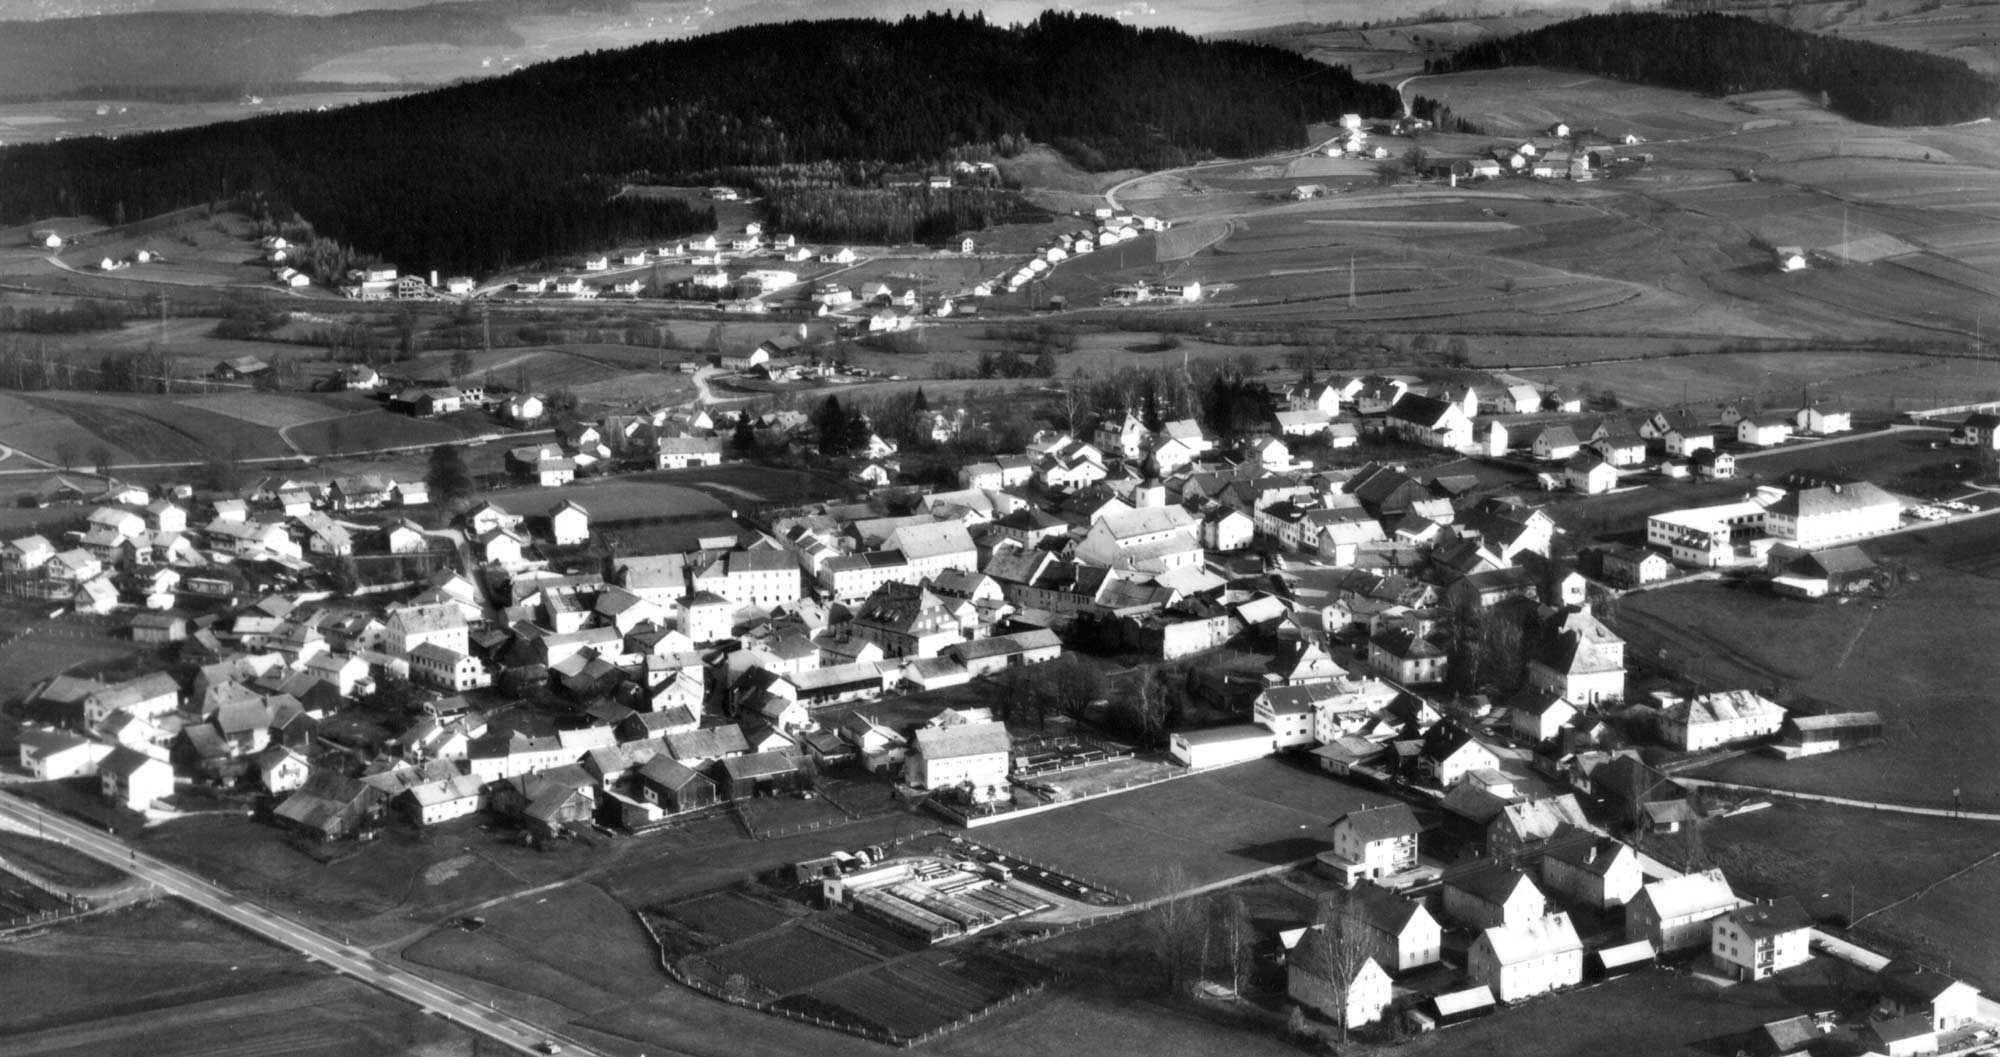
\includegraphics[width=15.981cm,height=8.446cm]{pictures/zulassungsarbeit-img016.jpg}


Ruhmannsfelden zur Zeit August Högns

Man kann davon ausgehen, dass Högn Ruhmannsfelden als einen
fortschrittlichen Ort erlebt hat, da dort kurz vor seiner Ankunft
Investitionen getätigt und Reformen durchgeführt wurden. So besaß
Ruhmannsfelden seit dem Schulhausneubau im Jahr 1908 (Abb. 16) gleich
drei Schulhäuser. \footnote{Reicheneder-Chronik, Schulwesen, Blatt 76
Vorderseite} Das älteste, 1834 erbaute Schulhaus (Abb. 15) konnte als
Lehrerwohnhaus genutzt werden und bot somit der jungen Familie eine
Wohnmöglichkeit. \footnote{Reicheneder-Chronik, Schulwesen, Blatt 68
Vorderseite} Auch in institutioneller Hinsicht hatte sich an der
Volksschule Ruhmannsfelden kurz vor 1910 Einiges geändert. Dem
Anwachsen der Schülerzahl wurde Rechnung getragen und statt früher vier
unterrichten nun sieben Lehrer, also ein Lehrer pro Schülerjahrgang.
Den jahrgangsübergreifenden und nach Geschlechtern getrennten Klassen
war somit ein Ende gesetzt. Die gemischten Jahrgänge umfassten aber
immer noch fast durchschnittlich 70 Schüler.\footnote{
Reicheneder-Chronik, Schulwesen, Blatt 16 Rückseite} 1908 hatten die
Anträge der Gemeinden Zachenberg und Patersdorf auf Einführung einer
Sommerschule Erfolg. Damit Kinder vor allem zur Erntezeit in der
Landwirtschaft ihrer Eltern mithelfen konnten, wurde vom 1. Mai bis 1.
Oktober ein auf drei Stunden verkürzter Unterricht
eingeführt. \footnote{Reicheneder-Chronik, Schulwesen, Blatt 8
Vorderseite}

\begin{flushleft}
\tablefirsthead{}
\tablehead{}
\tabletail{}
\tablelasttail{}
\begin{supertabular}{m{6.452cm}m{9.653cm}}

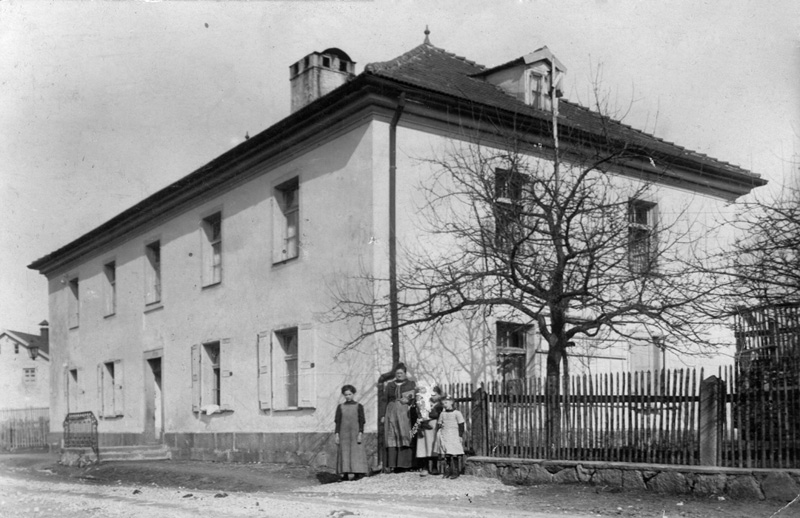
\includegraphics[width=6.269cm,height=3.999cm]{pictures/zulassungsarbeit-img017.jpg}

Schulhaus von
1834, ab 1908 als Lehrerwohnhaus genutzt &

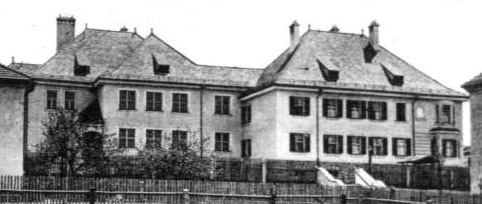
\includegraphics[width=9.47cm,height=4.001cm]{pictures/zulassungsarbeit-img018.jpg}

Schulhaus von
1908\\
\end{supertabular}
\end{flushleft}
Mit August Högn traten gleich drei neue Lehrer in Ruhmannsfelden ihren
Schuldienst an. In der Schulchronik wird Högn bald als 2. Lehrer und
somit Stellvertreter von Schulleiter Alois Auer aufgeführt.\footnote{
Volksschul-Chronik} Das hatte neben seiner schon 10 Jahre langen
Berufserfahrung wahrscheinlich auch den Grund, dass Högn die einzige
männliche Lehrerkraft neben Bezirksoberlehrer Auer war, die in den
unruhigen Zeiten des 1. Weltkrieges seiner neuen Heimat treu bleiben
konnte. Högns Kriegseinsatz beschränkte sich auf einen kurzen
Heeresdienst im Jahr 1915, bei dem er sich den König-Ludwig-Orden und
das Militär-Verdienstkreuz erwarb.

Eine weitere Neuerung war, dass die Pfarrkirche St. Laurentius im selben
Jahr, als August Högn nach Ruhmannsfelden kam, eine neue, pneumatische
Orgel mit 22 Registern vom Orgelbaumeister Ludwig Edenhofer aus
Deggendorf bekam. \footnote{Reicheneder-Chronik, Orgel, Blatt 74
Rückseite} Von Anfang an wirkte Högn an der Kirchenmusik in
Ruhmannsfelden mit. \footnote{Dokument Nr. 18, Brief von August Högn an
Pfarrer Reicheneder, 25.1.1954} Der versierte Orgelspieler\footnote{
Interview Nr. 16, Maria Freisinger, 25.8.2004, Absatz 28} war auch im
Kirchendienst mehr als ein würdiger Stellvertreter für Auer, der
zusammen mit seiner Frau Anna und Tochter Auguste den
Chorregentendienst ausführte.

Bereits ein halbes Jahr nach seiner Ankunft wurde Högn zum Vorstand
eines Ruhmannsfeldener Vereins gewählt, was seine schnelle
gesellschaftliche Integration in Ruhmannsfelden unterstreicht. Der
Turnverein Ruhmannsfelden suchte zu dem Zeitpunkt händeringend eine
Person, die sich bereit erklärte, den unbesetzten Posten des Vorstands
zu übernehmen. Vom 21.5.1910 \footnote{Dokument Nr. 101, Protokoll der
Turnvereinsversammlung, 21.5.1910}  bis 27.12.1913 \footnote{Dokument
Nr. 103, Protokoll der Turnvereinsversammlung, 27.12.1913} hatte Högn
dieses Amt inne. Auch wenn er nach dieser Zeit in keiner Funktion der
Vereinsspitze in Erscheinung tritt, blieb er trotzdem über Jahrzehnte
hinweg vor allem als Leiter der Sänger- und Orchesterriege dem Verein
treu. 1924 versuchte man noch einmal Högn in die Vereinsspitze als
Schriftführer mit einzubinden, doch er lehnte wahrscheinlich deswegen
ab, weil er schon bei der Ruhmannsfeldener Feuerwehr die
Schriftführertätigkeit ausübte. \footnote{Dokument Nr. 107, Protokoll
der Turnvereinsversammlung, 23.1.1924}

August Högn war bereits am 19.9.1902 der Wallersdorfer Feuerwehr
beigetreten \footnote{Dokument Nr. 110, Abschiedsrede des
Feuerwehrkommandanten Johann Linsmeier auf August Högn, 3.11.1951} und
wechselte Anfang Januar 1910 in die Feuerwehr Ruhmannsfelden. Am
26.12.1910 wurde Högn dann zum Schriftführer der Feuerwehr
Ruhmannsfelden gewählt. \footnote{Dokument Nr. 93, Protokoll der
Feuerwehrgeneralversammlung, 26.12.1910} Dass ein Lehrer den
Schriftführerposten der Feuerwehr übernahm, hatte in Ruhmannsfelden
Tradition. Die Lehrer Raymund Schinagl und Max Weig waren lange Zeit
vor Högn als Schriftführer tätig. Der Feuerwehr-Mitbegründer und letzte
Schriftführer Joseph Lukas starb am 30.8.1910, \footnote{Högn,
Feuerwehr, Blatt 7 b, Blatt 17, Blatt 34} sodass sein Posten frei
wurde. August Högn, als Lehrer im Schreiben souverän wie sonst kein
anderer bei der Feuerwehr, bot sich als Nachfolger für Lukas gerade zu
an. Die Protokolle vor Högns Zeit als Schriftführer zeichnen sich
dementsprechend durch viele Rechtschreibfehler aus.\footnote{
Feuerwehr-Protokoll} August Högn blieb 40 Jahre lang Schriftführer der
Feuerwehr. Neben dem Verfassen von Protokollen übernahm er die
Korrespondenz der Feuerwehr, hielt zahlreiche Ansprachen und Vorträge
und packte auch mal mit eigenen Händen an, als zum Beispiel 1933 bei
strömenden Regen die neue Feuerwehrspritze vom Zug abgeladen werden
musste. \footnote{Högn, Feuerwehr, Blatt 44, Blatt 46, Blatt 47, Blatt
54, Blatt 56}

Ein weiteres Aufgabenfeld, das die damalige dörfliche Gemeinschaft für
einen Lehrer bereithielt, übernahm August Högn 1913: Bis 1920 war
August Högn Gemeindeschreiber der Gemeinde Zachenberg. \footnote{Högn,
Zachenberg, Blatt 16} Nach dem Erlass der Gemeindeverordnung wurden
diese Arbeiten hauptsächlich den Lehrern übertragen. \footnote{Geyer,
Seite 106} So verwundert es nicht, dass die angehenden Lehrer in den
Lehrerbildungsanstalten speziell im Fach Gemeindeschreiberei
unterrichtet wurden \footnote{Dantl, Seite 82} und dass vor Högn die
Lehrer Milter, Schinagl, Lechner und Hochstraßer für die Gemeinde
Zachenberg tätig waren. \footnote{Högn, Zachenberg, Blatt 11, Blatt 15,
Blatt 16} Högns Eifer, sich für das Gemeinwohl zu engagieren, kommt
auch dadurch besonders zum Ausdruck, dass er sogar ein Zimmer seiner
Dienstwohnung abtrat und es in eine Art Gemeindekanzlei
umwandelte.Vorher wurden die
Gemeindearbeiten, die für Lehrer eine wichtige Nebeneinkunft
darstellten, in einem Raum der Brauerei Rankl in Ruhmannsfelden
erledigt.
